\section{泊肃叶流}

\begin{frame}
    \begin{figure}[H]
        \centering
        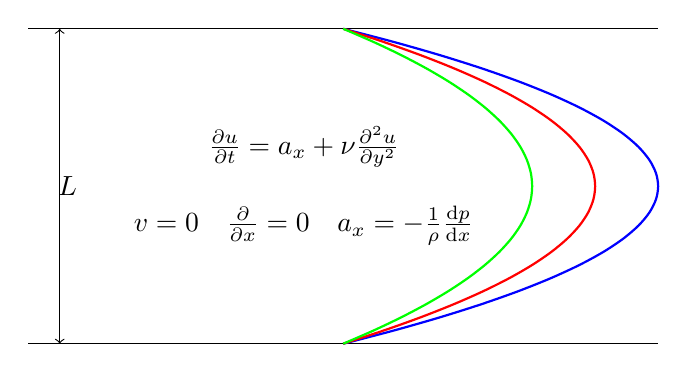
\begin{tikzpicture}
            \def\pipediameter{4}
            \def\pipelength{8}
            \draw (0,0) -- (\pipelength,0);
            \draw (0,\pipediameter) -- (\pipelength,\pipediameter);

            % \draw a y(L-y) = x inside the pipe
            % flow's shape
            \draw[domain=0:\pipediameter,smooth,variable=\y,blue,thick=3] plot ({4+\y*(\pipediameter-\y)},{\y});
            \draw[domain=0:\pipediameter,smooth,variable=\y,red,thick=3] plot ({4+0.8*\y*(\pipediameter-\y)},{\y});
            \draw[domain=0:\pipediameter,smooth,variable=\y,green,thick=3] plot ({4+0.6*\y*(\pipediameter-\y)},{\y});
            
            % governing equation
            \node at (3.5,2.5) {$\frac{\partial u}{\partial t}  = a_x + \nu\frac{\partial^2 u}{\partial y^2}$};
            \node at (3.5,1.5) {$v=0\quad\frac{\partial }{\partial x}=0\quad a_x=-\frac{1}{\rho}\frac{\mathrm{d}p}{\mathrm{d}x}$};

            % L
            \node at (0.5, 0.5*\pipediameter) {$L$};
            \draw[<->] (0.4,0) -- (0.4,\pipediameter);
        \end{tikzpicture}
    \end{figure}
    级数解 (Morris):
    \begin{equation}
        \begin{aligned}
            u(y,t)
        &=
        \frac{a_x}{2\nu}y(L-y)\\
        &-
        \sum_{k=0}^{\infty}
        \frac{2a_xL^2}{\nu\pi^3(2k+1)^3}
        \sin\left(\frac{\pi(2k+1)y}{L}\right)
        \exp\left(-\frac{\pi^2(2k+1)^2\nu t}{L^2}\right)
        \end{aligned}
    \end{equation}
\end{frame}

\begin{frame}
    \begin{figure}[H]
        \centering
        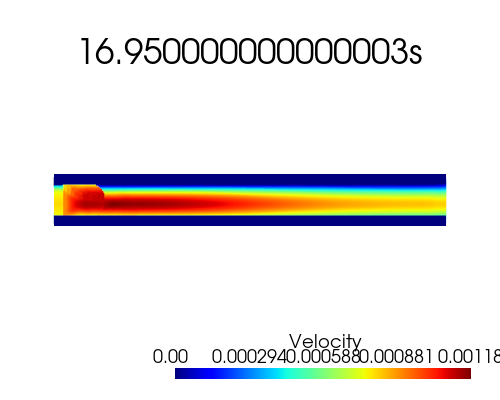
\includegraphics[width=0.8\textwidth]{images/Poiseuille2D/poiseuille_2d.png}
    \end{figure}
\end{frame}

\begin{frame}
    对于这种开边界问题,
    最常用的是采用“粒子缓冲区”技术进行处理。
    \begin{figure}[H]
        \centering
        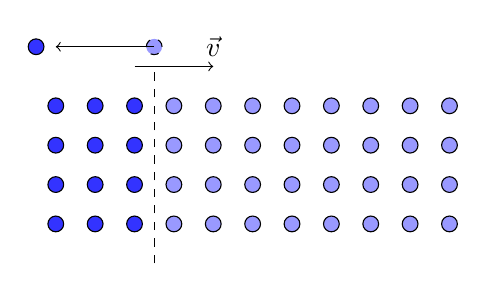
\begin{tikzpicture}
            % calculation domain
            % 8 * 4 particles
            % dx = 0.5
            \def\dx{0.5}
            \foreach \x in {0,1,...,7}
            \foreach \y in {0,1,...,3}
            \filldraw[fill=blue!40!white,draw=black] ({\x*\dx},{\y*\dx}) circle (0.1);
            % left inlet buffer
            \foreach \x in {-1,-2,-3}
            \foreach \y in {0,1,...,3}
            \filldraw[fill=blue!80!white,draw=black] ({\x*\dx},{\y*\dx}) circle (0.1);

            \draw[dashed] ({-\dx/2}, -\dx) -- ({-\dx/2}, 4*\dx);

            \draw[->] (-\dx, {4*\dx}) -- (\dx, {4*\dx}) node[above] {$\vec{v}$};

            % draw a particle pass into calcilation domain with dashed line
            \filldraw[fill=blue!40!white,draw=black,dashed] ({-\dx/2},{4.5*\dx}) circle (0.1);
            % draw a circle line to let the particle back to the buffer
            \draw[->] ({-\dx/2},{4.5*\dx}) -- ({-\dx/2-2.5*\dx},{4.5*\dx});
            \filldraw[fill=blue!80!white,draw=black] ({-\dx/2-3*\dx},{4.5*\dx}) circle (0.1);
        \end{tikzpicture}
    \end{figure}
    一旦 inlet 流入区域的粒子跨过了缓冲区的边界,
    则将其实例化成一个新流体粒子纳入计算区域。
    而将其位置重新沿流向,上溯缓冲区的宽度的距离,
    重新放入缓冲区。
    而另一方面流出区域的粒子则直接删除,也会有一个 outlet 缓冲区。

    因此泊肃叶流中,
    需要有:壁面粒子,流入缓冲区粒子,计算区域粒子,流出缓冲区粒子。
\end{frame}

\begin{frame}
    \begin{figure}[H]
        \centering
        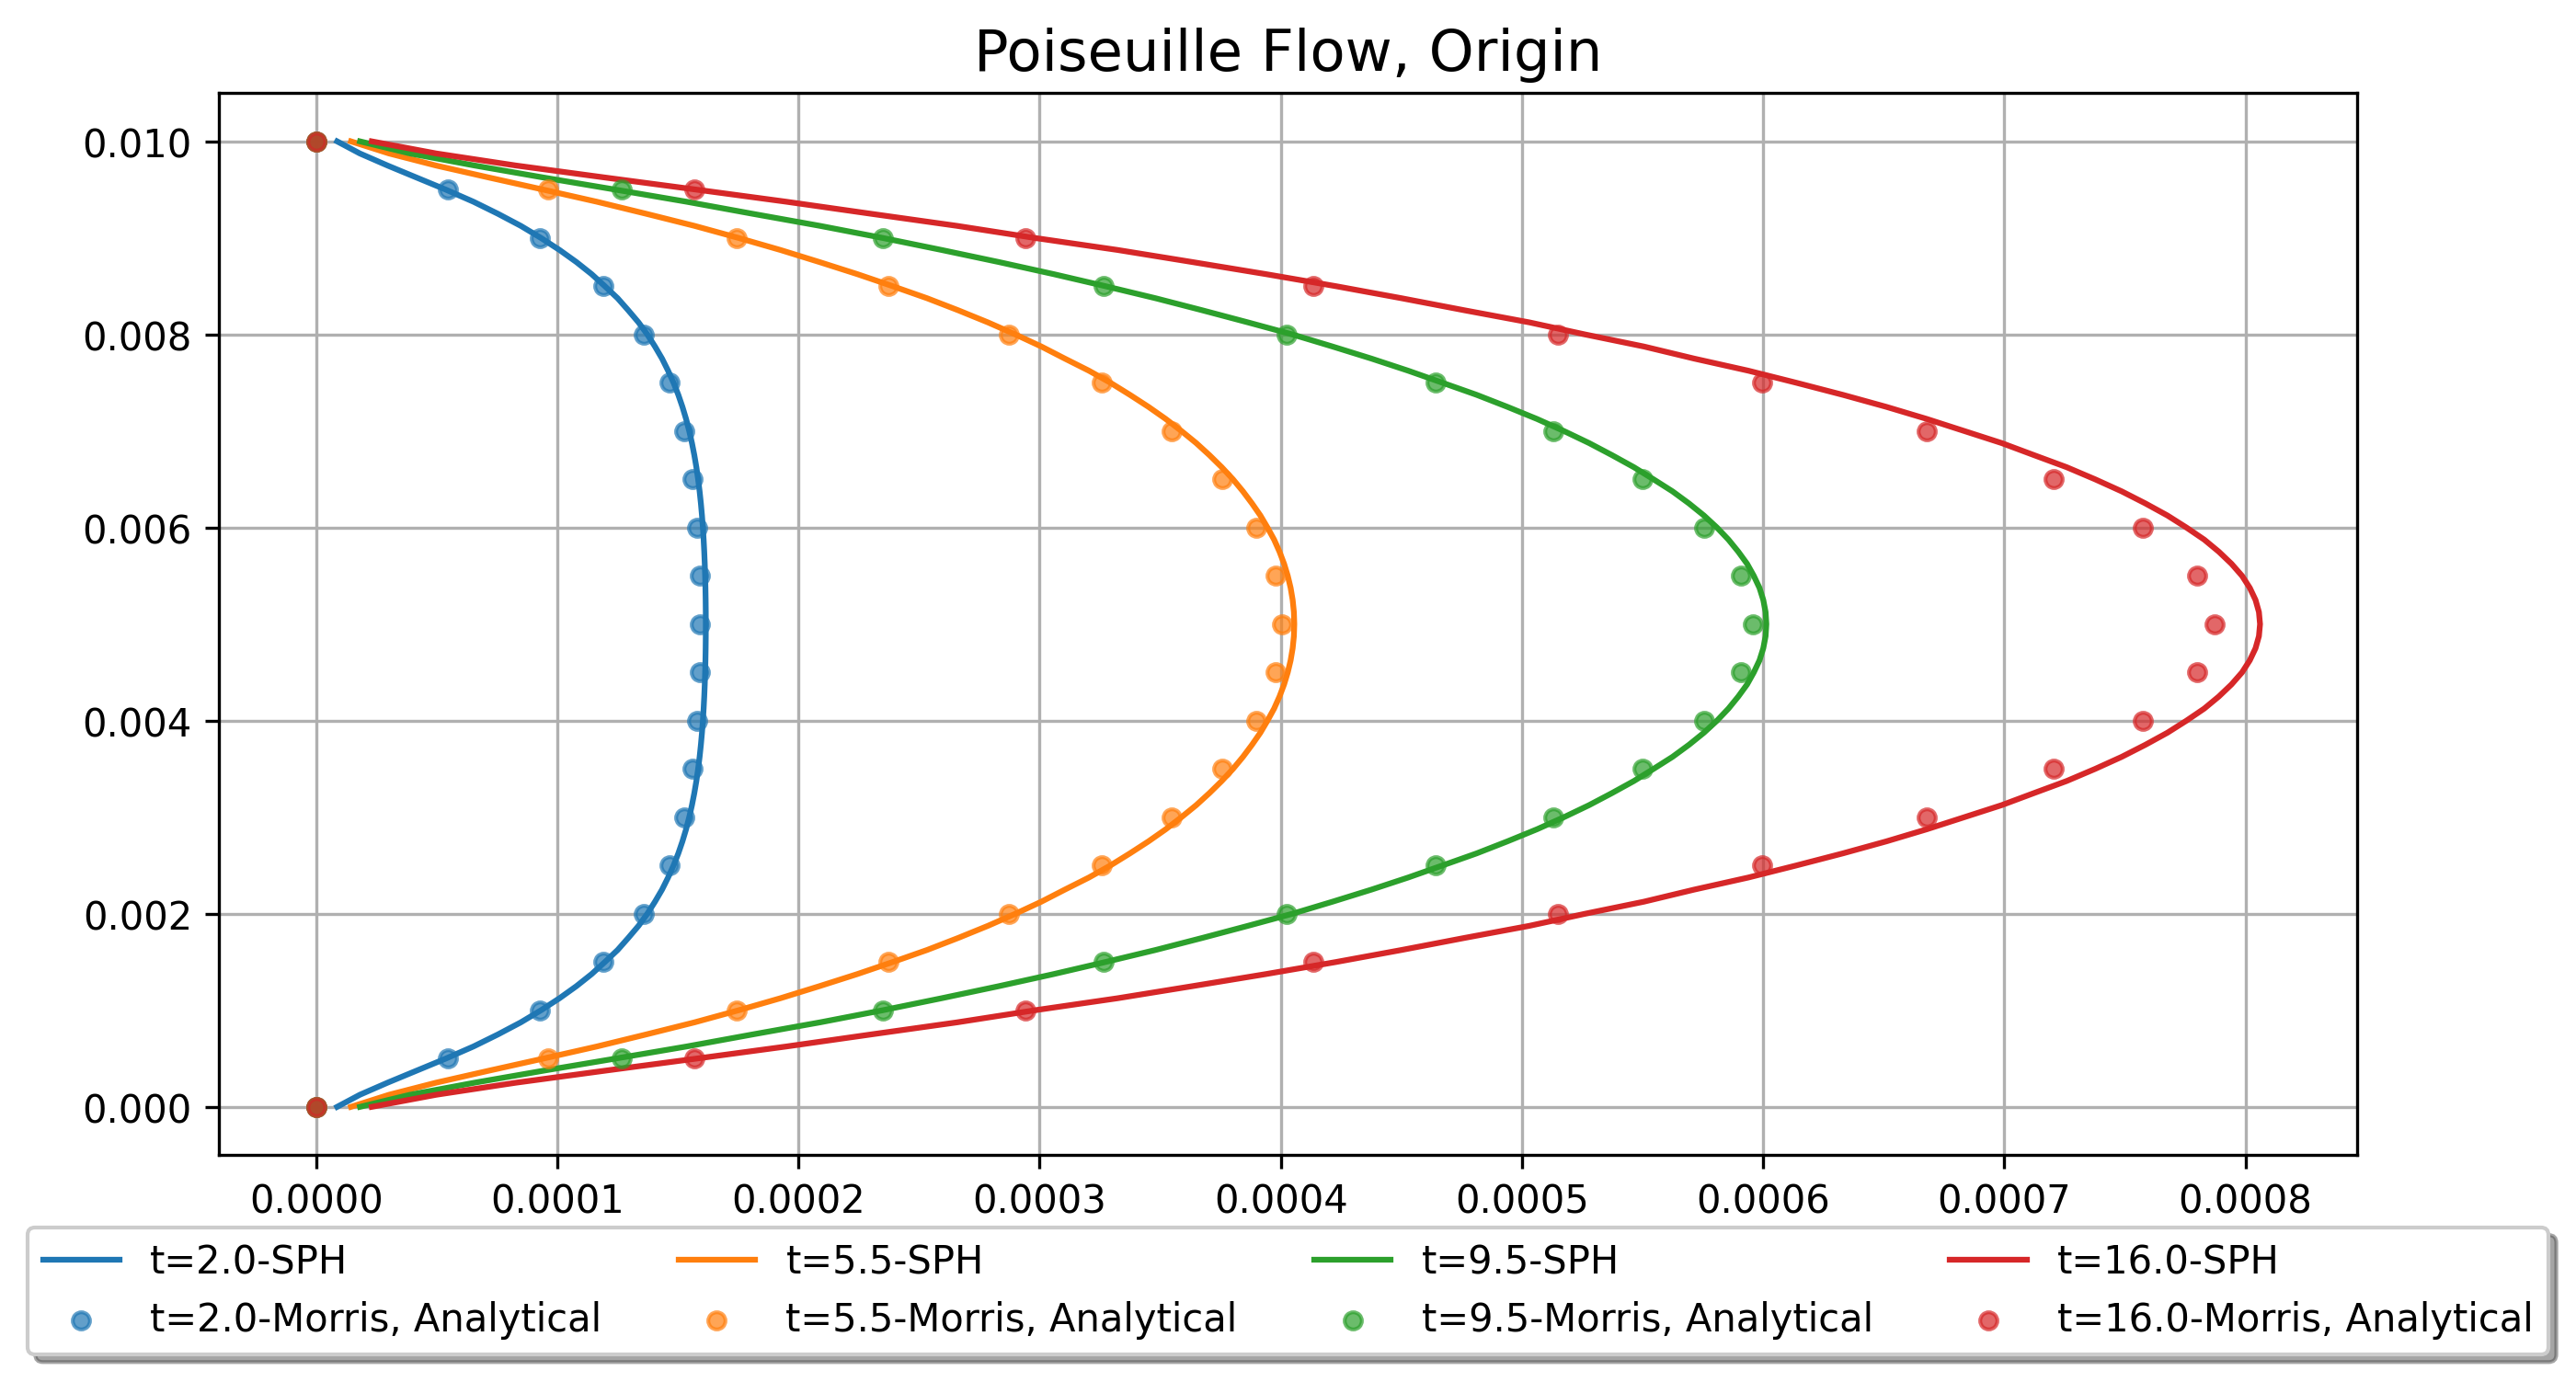
\includegraphics[width=\textwidth]{images/Poiseuille2D/poiseuille_2d_origin.png}
        \caption{未垫高壁面粒子的泊肃叶流}
    \end{figure}
\end{frame}

\begin{frame}
    \begin{figure}[H]
        \centering
        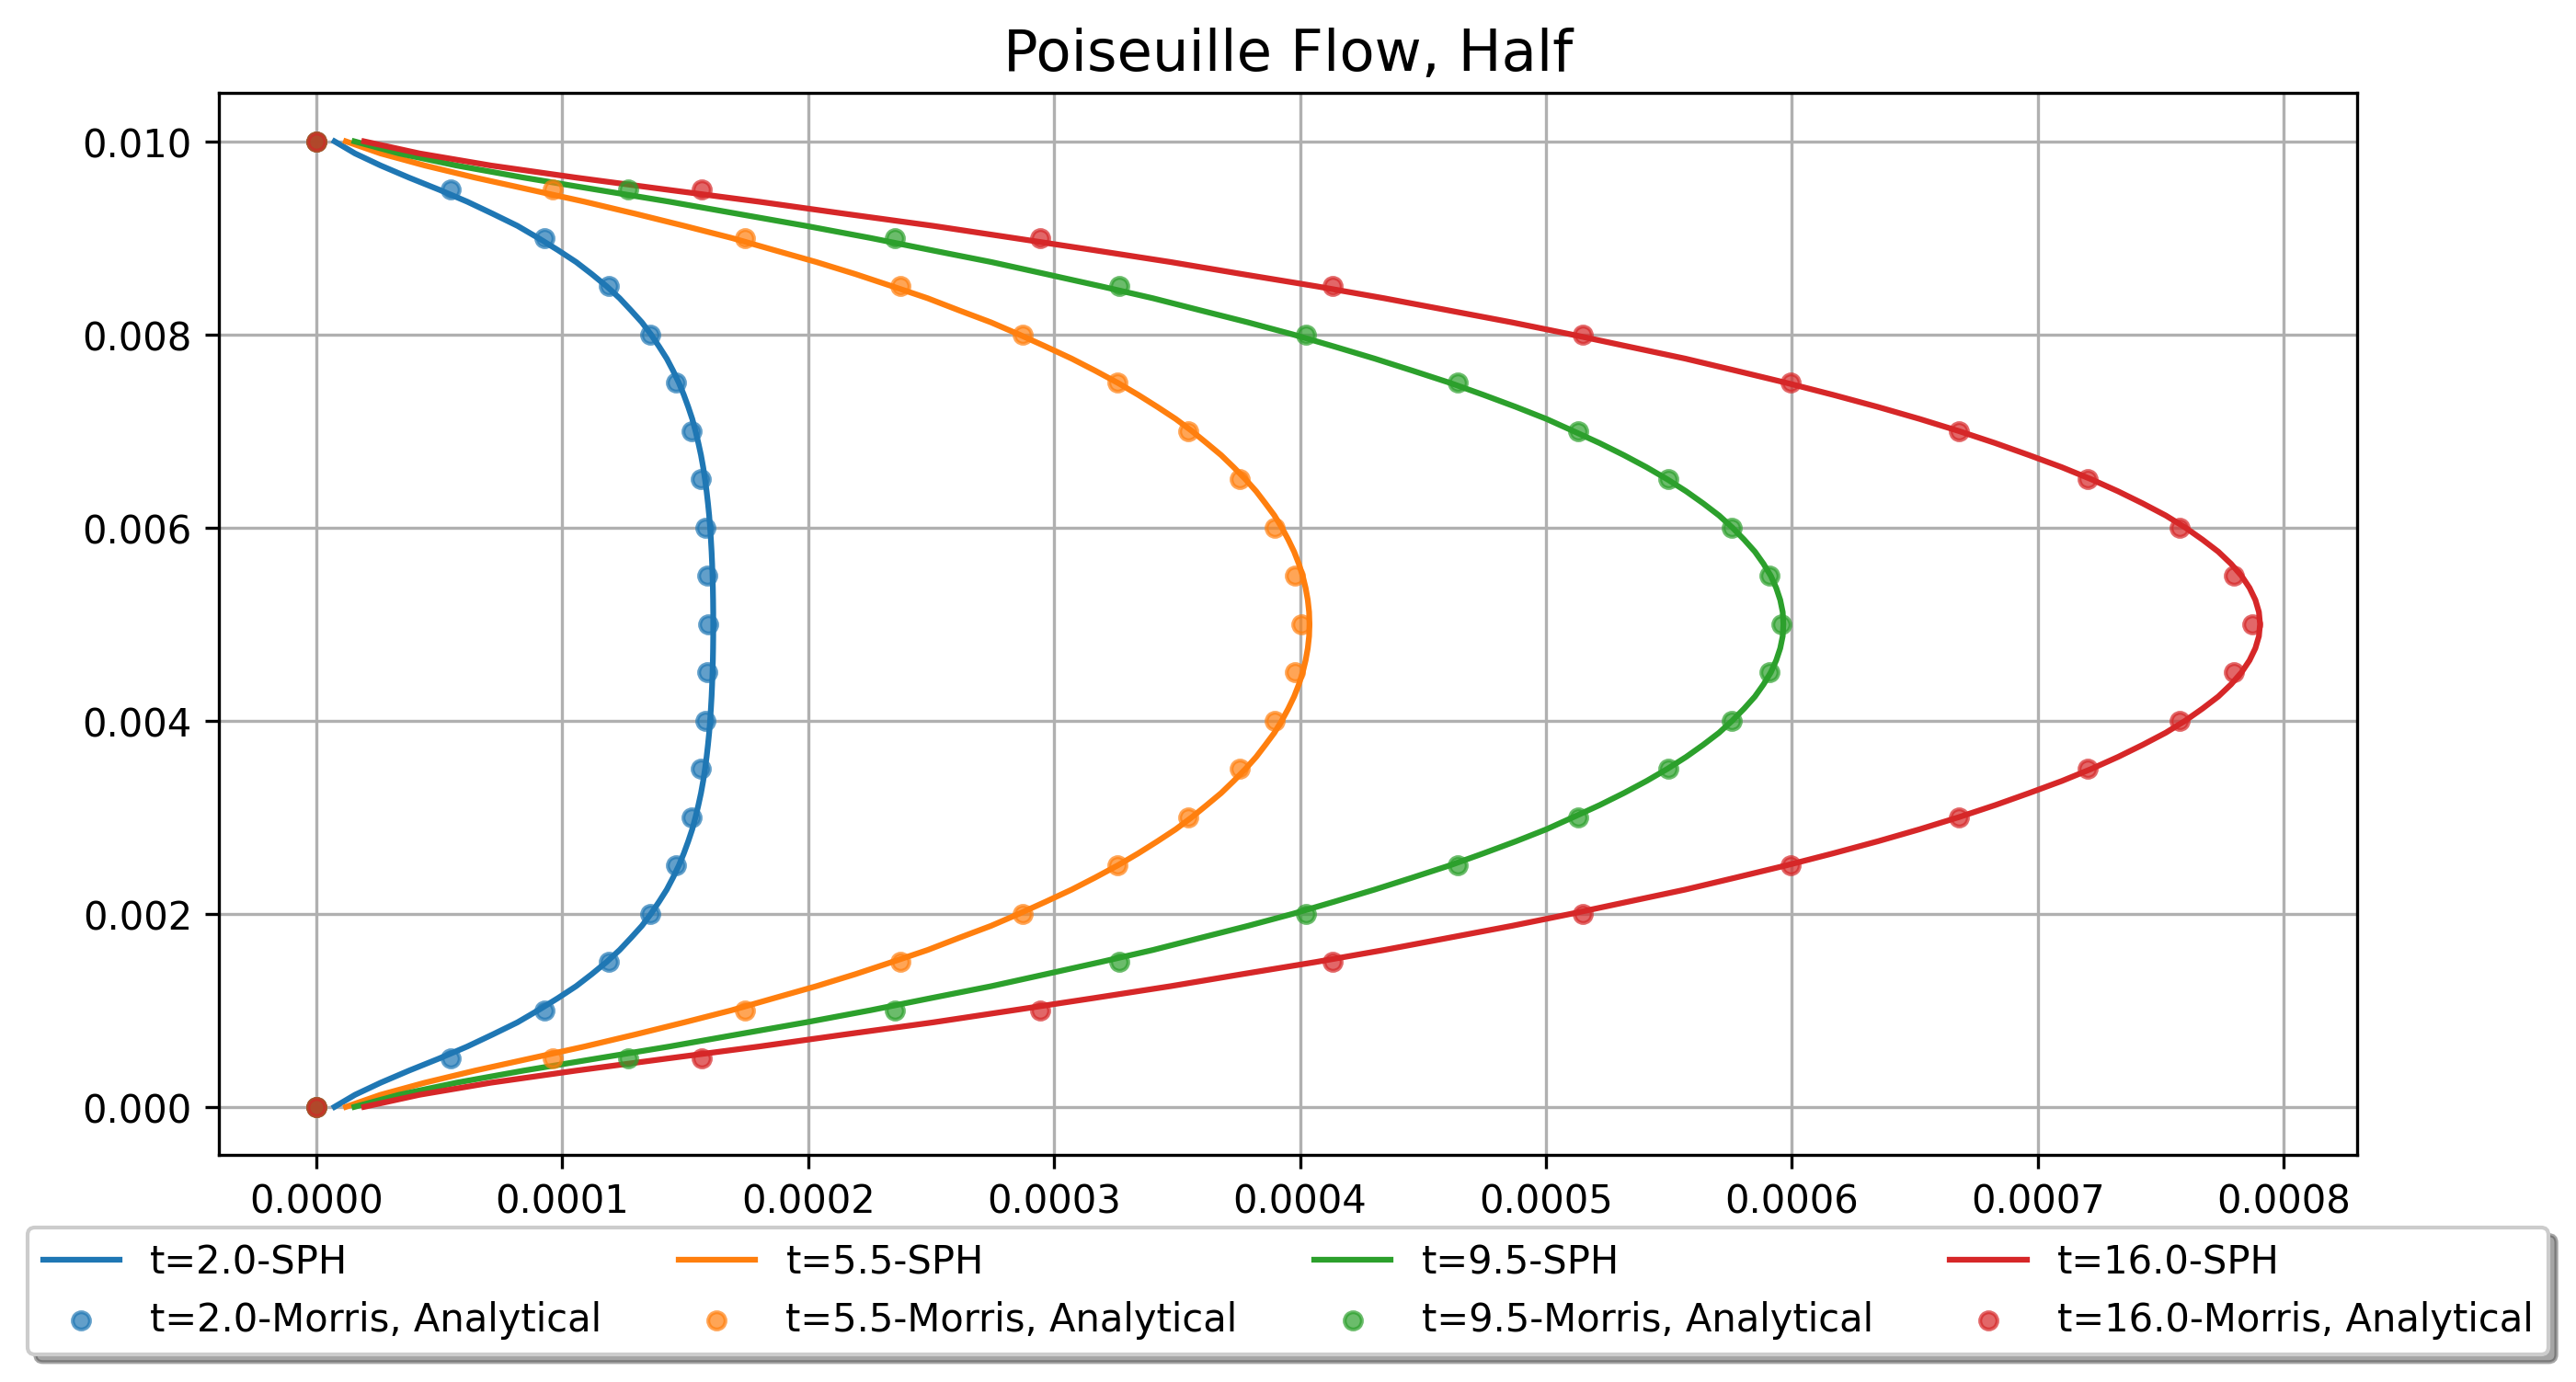
\includegraphics[width=\textwidth]{images/Poiseuille2D/poiseuille_2d_half.png}
        \caption{垫高壁面粒子的泊肃叶流}
    \end{figure}
\end{frame}

\begin{frame}
    通过泊肃叶流这个算例,
    可以发现垫高壁面粒子可以取得
    与理论解析解更加吻合的结果。
    
    但是似乎在顶盖驱动流算例中却不是这样的。

    对于壁面摩擦这件事情,
    我查的论文中对粘性项的讨论都莫衷一是,
    而且 Monaghan 本人也认为 SPH 中的壁面条件是一个并没有完全解决的问题。
    (包括开边界中如何正确利用黎曼条件)。
    不过至少目前看来,
    垫高壁面粒子是一个可行的方案。
\end{frame}